\documentclass[a4paper, 10pt, titlepage]{article}

\usepackage{listings}
\usepackage{newclude}
\usepackage{subfigure}
\usepackage{color}
\usepackage{amsmath}
\usepackage[utf8]{inputenc}
\usepackage{graphicx}

\definecolor{dkgreen}{rgb}{0,0.6,0}
\definecolor{gray}{rgb}{0.5,0.5,0.5}
\definecolor{mauve}{rgb}{0.58,0,0.82}

\lstset{	% must add \usepackage{listings}
  language=C,	  % the language of the code
  basicstyle=\footnotesize, % the size of the fonts that are used for the code
  numbers=left,	    % where to put the line-numbers
  numberstyle=\tiny\color{gray},  % the style that is used for the line-numbers
  stepnumber=1,	    % the step between two line-numbers. If it's 1, each line will be numbered
  numbersep=5pt,      % how far the line-numbers are from the code
  backgroundcolor=\color{white},% choose the background color. You must add \usepackage{color}
  showspaces=false,   % show spaces adding particular underscores
  showstringspaces=false,   % underline spaces within strings
  showtabs=false,     % show tabs within strings adding particular underscores
  frame=l,	  % adds a frame around the code
  rulecolor=\color{black},    % if not set, the frame-color may be changed on line-breaks within not-black text (e.g. commens (green here))
  tabsize=4,	    % sets default tabsize to 2 spaces
  captionpos=b,	    % sets the caption-position to bottom
  breaklines=true,	% sets automatic line breaking
  breakatwhitespace=false,  % sets if automatic breaks should only happen at whitespace
  title=\lstname,     % show the filename of files included with \lstinputlisting; also try caption instead of title
  keywordstyle=\color{blue},  % keyword style
  commentstyle=\color{dkgreen},% comment style
  stringstyle=\color{mauve},  % string literal style
  escapeinside={\%*}{*)}, % if you want to add a comment within your code
  morekeywords={*,...}	  % if you want to add more keywords to the set
}


\title{Assignment TDT4258 Assignment 3 - Group 1}
\author{Sondre Lefsaker
  \and André Philipp
  \and Håvard Wormdal Høiby}

\begin{document}
  \maketitle
  \newpage

  \section{Abstract}

  \tableofcontents
  \section{Introduction}
The second assignment introduces us to a new hardware device, the ABDAC. We also utilize
the buttons and LEDs used in assignment one. This gives an introduction to programming with
audio devices and how to produce audio digitally.\\
\\
To the development environment from assignment one we add the GCC C-compiler.\\
\\
The gist of this assignment is to produce different sounds when the buttons on the board are pressed.
The program should be implemented in the C programming language without the support of an
Operation System. We implemented two modes. The first mode is a 7-note piano. The second is a
playback function which plays a different predefined sample for each button. The button SW0
is used to toggle between the two modes.\\
\\
In order to make the program energy efficient the CPU is set to sleep and the DAC is shut 
down while nothing is playing. %a tone is not playing.


  \include*{setup}
  \include*{setup/board}
  \include*{setup/sound}
  \include*{setup/game}

  \section{Overview}

  \include*{overview/drivers}
  \subsection{Graphics}

\subsubsection{Screen}

The screen is opened and memory mapped in the {\bf Screen} object like this.
\\
\begin{lstlisting}
  int fd = screen->_fd = open( "/dev/fb0", ... );
  screen->frame_buffer = (uint8_t*)mmap( 0, SCREEN_SIZE, ... , MAP_SHARED, fd, 0 );
\end{lstlisting}
The screen has a method {\bf ScreenFlush} to flush the whole internal buffer into the frame buffer:
\\
\begin{lstlisting}
  void ScreenFlush( Screen *screen ) {

    for (int i=0; i < SCREEN_SIZE; i++) {
      screen->frame_buffer[i] = screen->internal_buffer[i];
    }

  }
\end{lstlisting}
To draw to the internal buffer it supplies the {\bf ScreenDrawPixel} method:
\\
\begin{lstlisting}

  void ScreenDrawPixel(Screen *screen, int x, int y, Pixel *pixel) {

    if (x >= 0 && x < screen->width && y >= 0 && y < screen->height) {
      if (PixelNotTransparant(pixel)) {
	int coordinate = y * screen->width * 3 + x * 3;
	*((Pixel*)&screen->internal_buffer[coordinate]) = *pixel;
      }
    }
  }
\end{lstlisting}
The {\bf PixelNotTransparant} function lets us paint pictures with
transparency. If it returns {\bf false} the pixel is simply not drawn.
The function also does boundry checks to make sure that the pixel is
on the screen. This helps the graphical objects to not care about
whether they
are on the screen or not in their paint method.

\subsubsection{Canvas}
The {\bf CanvasPaint} method is found in the core of the {\bf Canvas} object.
It is reponsible for drawing each graphical object on to the
screen. This loop runs though all objects and ask them to paint themselves
 on the screen.
\\
\begin{lstlisting}
  for (int i=0; i<canvas->top; i++) {
    if (canvas->shapes[i]) {
      Shape *shape = (Shape*)canvas->shapes[i];

      (*((Shape*)shape)->paint)( canvas->shapes[i], screen );
    }
  }
\end{lstlisting}
Afterwards, the method asks the {\bf Screen} object to update the screen
buffer through the {\bf ScreenFlush} method.

\subsubsection{Shape}
The {\bf Shape} exists only to provide a structure for which other
graphical objects shall match. In this implementation the most
importaint part is the {\bf paint} function pointer, which all
graphical object must have as their second member. The first member is
a pointer to the objects parent. This is only used for the {\bf Bitmap}
type.
\\
\begin{lstlisting}
  typedef struct {
    void *parent;
    void (*paint) ( void*, Screen* );
    int x;
    int y;
    void *child;
  } Shape;
\end{lstlisting}

\subsubsection{Image}
The {\bf Image} object is only an abstract object, its responsibility
is to conseal the implemented file format. Therefore, its implementetion
is fairly simple. The {\bf paint} method delegates all its work to the
format specific object.
\\
\begin{lstlisting}
  static void paint (void *shape, Screen *screen) {

    Image *image = (Image*) shape;
    Shape *actual_image = (Shape*)image->image;
    actual_image->paint( actual_image, screen  );

  }
\end{lstlisting}

\subsubsection{Bitmap}
The {\bf Bitmap} object is by far the most complex object in the
graphics module. It is responsible for reading the bitmap fileformat
and rendering its contents in the internal buffer. The reading is
implemented in three steps.

\begin{enumerate}
\item Reading the file header \newline
  The file header is read directly into the {\bf BMPHeader} structure.
  \begin{lstlisting}
    static BMPHeader ReadBMPHeader ( int fd ) {

      BMPHeader header;
      read( fd, &header, sizeof(header));

      return header;
    }
  \end{lstlisting}

\item Reading the DIB header \newline
  We only need the first three fields of the DIB header, these are read
  into the struct.
  \begin{lstlisting}
    static DIBHeader ReadDIBHeader ( int fd ) {

      DIBHeader header;
      read( fd, &header, sizeof(header));
      return header;
    }
  \end{lstlisting}

\item Converting endian of the file header \newline
  The fileformat headers are written in little-endian, the Linux on the
  board uses big-endian. This is fixed with a bit of byte swapping.
  \begin{lstlisting}
    static void fix_endian( BMPHeader *bmp_header, DIBHeader *dib_header ) {

      char *p;

      // BMP header
      p = (char*) &bmp_header->signature;
      swap( &p[0], &p[1] );

      p = (char*) &bmp_header->size;
      swap( &p[0], &p[3] );
      swap( &p[1], &p[2] );

      p = (char*) &bmp_header->reserved1;
      swap( &p[0], &p[1] );

      p = (char*) &bmp_header->reserved1;
      swap( &p[0], &p[1] );

      p = (char*) &bmp_header->offset;
      swap( &p[0], &p[3] );
      swap( &p[1], &p[2] );

      // DIB header
      p = (char*) &dib_header->size;
      swap( &p[0], &p[3] );
      swap( &p[1], &p[2] );

      p = (char*) &dib_header->width;
      swap( &p[0], &p[3] );
      swap( &p[1], &p[2] );

      p = (char*) &dib_header->height;
      swap( &p[0], &p[3] );
      swap( &p[1], &p[2] );

    }
  \end{lstlisting}

\item Making sense of the headers
  \begin{lstlisting}
    int offset = bmp_header.offset;
    int size = bmp_header.size;
    int width = dib_header.width;
    int height = dib_header.height;
  \end{lstlisting}
\item Reading the content \newline
  The actual bitmap from the offset in the header untill the end of the
  file. All of this is read into the {\bf data} variable.
  \begin{lstlisting}
    uint8_t *data = malloc(size);
    uint8_t *ptr = (uint8_t*)data;

    for (int i=0; i < (size - offset) / BUFFER_SIZE; i++ ) {
      read( fd, buffer, BUFFER_SIZE );

      for (int i=0; i<BUFFER_SIZE; i++) {
	(*ptr++) = buffer[i];
      }
    }

    int remaining = (size - offset) % BUFFER_SIZE;
    if (remaining) {
      read( fd, buffer, remaining);

      for (int i=0; i<remaining; i++) {

	(*ptr++) = buffer[i];
      }
    }
  \end{lstlisting}

  \item Flipping the rows of the content \newline
The rows in the bitmap array is stored in the wrong order so
we have to flip them over.
    \begin{lstlisting}
      static void swapLine ( uint8_t *a, uint8_t *b, int width ) {

	for (int i=0; i<width; i++) {
	  swap(&a[i], &b[i]);
	}

      for (int i=0; i<width; i++) {
	swap(&a[i], &b[i]);
      }

    }

    static void flip ( uint8_t *data, int width, int height ) {

      for (int i=0, j=height-1 ; i < height/2; i += 1, j -= 1) {
	swapLine( &data[i*width*3], &data[j*width*3], width*3 );
      }
    \end{lstlisting}
  \item Saving the useful data\newline
Now we only need the {\bf width}, {\bf height} and {\bf data} in order
to draw the image on the screen.
    \begin{lstlisting}
	bmp->width = width;
	bmp->height = height;
	bmp->pixels = data;
    \end{lstlisting}
\end{enumerate}
The {\bf paint} method of the {\bf Bitmap} object copies the pixel
values from its internal memory. It draws them on the screen with a
vertical and horizontal shift according to its parent, {\bf Image}, x
and y values. This enables the image to be painted at an arbitrary
place on the screen.
\\
\begin{lstlisting}
  static void paint ( void *shape, Screen *screen ) {

    Bitmap *image = (Bitmap*) shape;
    Image *parent = (Image*) image->parent;

    int sx = parent->x;
    int sy = parent->y;

    int width = image->width;
    int height = image->height;

    for (int y = 0; y < height; y++) {
      for (int x = 0; x < width; x++) {
	Pixel *p = &image->pixels[y*width + x];
	ScreenDrawPixel( screen, x+sx, y+sy, p);
      }
    }
  }
\end{lstlisting}

\subsubsection{Line}
The {\bf Line} object is responsible for drawing lines on the {\bf Screen}. It can be
used for making compound objects like rectangles and triangles. The paint method uses
Simplified Bresenham's line algorithm\footnote{http://en.wikipedia.org/wiki/Bresenham's\_line\_algorithm}.

\begin{lstlisting}
  while (1) {
    ScreenDrawPixel(screen, x0, y0, &pixel);
    if (x0 == x1 && y0 == y1) {
      break;
    }

    int e2 = 2*err;
    if (e2 > -dy) {
      err = err - dy;
      x0 = x0 + sx;
    }
    if (e2 < dy) {
      err = err + dx;
      y0 = y0 + sy;
    }
  }

\end{lstlisting}

\subsubsection{Rectangle}
The {\bf Rectangle} object uses the {\bf Line} object to draw a rectangle on the {\bf Screen}.
\begin{lstlisting}
  static void paint ( void *shape, Screen *screen ) {

    Rectangle *rect = (Rectangle*)shape;

    int x = rect->x;
    int y = rect->y;
    int dx = rect->dx;
    int dy = rect->dy;

    Line l1 = LineNew(x, y, dx, 0);
    l1.paint( &l1, screen );

    Line l2 = LineNew(x, y+dy, dx, 0);
    l2.paint( &l2, screen );

    Line l3 = LineNew(x, y, 0, dy);
    l3.paint( &l3, screen );

    Line l4 = LineNew(x+dx, y, 0, dy);
    l4.paint( &l4, screen );
  }
\end{lstlisting}

  \subsection{Sound}
\label{sec:alsa}

In order to have audible sound on the board the sound setting in Linux must be set correctly.

This can be done by opening the alsamixer (execute {\bf alsamixer} as root at the shell prompt).
Here all items should be unmuted, select the item with the arrows and unmute with the {\bf m} key.
The items must also be set to appropiate levels, the levels are set with the arrow keys. Exit
the program with the {\bf ESC} key.

  \subsection{Game}
The game was simply tested during development, the iterative process of implementing
small parts and testing them, eventually led to a fully working game. There are 
mainly three things that should work;
\begin{enumerate}
  \item Player A should be able to move the tank
  \item Player B should be able to move the cannon aim
  \item The round should end in favour to player A if the tank reaches the turret, or it
  	should end in favour to player B if the turret hits the tank.
\end{enumerate}

\subsubsection{Tank movement}
The tank should be able to move in all four directions, and accross the whole field. The only 
restrictions is when trying to move out of the field (the bounds of the game) and when
trying to move over fire. When the tank enters the top right tile, i.e. the location of the 
turret, the round should end in favour to the tank. Thus the tank can find itself in four
different situations;
\begin{enumerate}
  \item Trying to move over open field
  \item Trying to move over fire
  \item Trying to move out of the field
  \item Trying to move on top of the turret
\end{enumerate}

\subsubsection{Turret movement}
The turret does not have the same controls as the tank, but it beahves almost the same. 
The main difference is the possibility to shoot anything execpt for itself. 
The turret can find itself in three different situations.
\begin{enumerate}
  \item Trying to aim over open field
  \item Trying to aim out of the field
  \item Shoot where it aims. It should not have any effect if it tries to shoot at fire
  or itself.
\end{enumerate}

\subsubsection{Ending the game}
A round should end when either player A has reached the turret, or player B has hit the tank.
Each player has four lives indicated by how many lights are lighting. When one player has won
four rounds the player should also have won the game (making the other player a looser), 
and the screen should display two different images depending on who won the game. There are
two different scenarios;
\begin{enumerate}
  \item Player A wins
  \item Player B wins
\end{enumerate}

\subsubsection{Test results}
We have tested all the previously listed situations for tank and turret, from two to four
different angles (depending on edges and corners of the field), and they all work
according to the expectations. \\
\\
We have also tested playing the game by winning four consecutive turns for player A and for 
player B, and we have tested different combinations of winning and losing rounds. 
The lights represenenting the remaining lives work as expected, and the game ends displaying
the correct image after a player has won four rounds.

  \section{Solution}
The following sections will describe the different parts of how we implemented the
different parts of the assignment.
\subsection{Button interrupts}
The \textbf{interrupt.c} file has two public functions that is called when an interrupt occurs;
the \textbf{button\_isr} function is called whenever a button is pressed, and
the \textbf{abdac\_isr} function is called regularely at the frequency of the assigned clock.\\
\\
The following code enables interrupts when the buttons is pressed, the first parameter to
the \textbf{register\_interrupt} is the interrupt routine. \\
\begin{lstlisting}
void init_buttons(void) {
	register_interrupt((__int_handler)(button_isr),
			   AVR32_PIOB_IRQ / 32, AVR32_PIOB_IRQ % 32, BUTTONS_INT_LEVEL);
	piob->per = 0xff;
	piob->ier = 0xff;
	piob->puer = 0xff;
}
\end{lstlisting}
The button\_isr function reads from the \textit{isr} register in order to find out what button
is pressed. If SW0 is pressed it switches mode, as described in the previous section,
otherwise it calls a handler function based on if the mode is PIANO\_MODE or PLAYBACK\_MODE.
\begin{lstlisting}
__int_handler *button_isr(void) {
	debounce();

	uint8_t button_interrupt = piob->isr;
	uint8_t button_down = ~(uint8_t)piob->pdsr;
	playing = button_down;

	if ( button_interrupt == SW0 ) {
		if (button_down)
			handle_mode_switch();
	} else {
		if (mode == PIANO_MODE)
			handle_piano_pressed(button_down, button_interrupt);
		else
			handle_sample_pressed(button_down, button_interrupt);
	}

	return 0;
}
\end{lstlisting}
The two handler function \textbf{handle\_piano\_pressed} and \textbf{handle\_sample\_pressed}
pretty much do the same thing; find out what button is pressed and
wake up the abdac if it is sleeping. The handle\_sample\_pressed also resets the currently
playing track (if any) and loads a new track based on the button that was pressed.

\subsection{Sound generation}
To generate sound we used the internal ABDAC (Audio Bitstream Digital-to-Audio-Converter)
on the AVR32 board. It takes a sequence of samples and converts it into an analog
signal, amplifies and outputs it.
The ABDAC uses 2 of the pins on the PIO port B to send signals to the output, and the
6th clock of the Power Manager to generate interrupts that processes the samples.
The clock is set up with oscillator 0 as the source and no division of the frequency.
This gives us a clock of 20 MHz and a sample rate of 20MHz / 256 = 81.920 kHz on the ABDAC\\
Details about these settings was found in the documentation\cite{avr32-stk1000}.
\begin{lstlisting}
	// Register interrupt handler
	register_interrupt((__int_handler)(abdac_isr),
			   AVR32_ABDAC_IRQ / 32, AVR32_ABDAC_IRQ % 32, ABDAC_INT_LEVEL);

	// Disable PIO
	piob->PDR.p20 = 1;
	piob->PDR.p21 = 1;

	// Enable ABDAC
	piob->ASR.p20 = 1;
	piob->ASR.p21 = 1;

	// Set the clock to use Oscillator (OSC0 and OSC1 is 20MHz and 12MHz)
	volatile avr32_pm_t *sm = &AVR32_PM;
	volatile avr32_pm_gcctrl_t *clock = &sm->gcctrl[6];

	clock->oscsel = 0;
	clock->pllsel = 0;
	clock->cen = ON;
\end{lstlisting}
The ABDAC is turned of when it is not used, to save power and keep the output silent.\\
\begin{lstlisting}
	dac->CR.en = OFF;
	dac->IER.tx_ready = OFF;
\end{lstlisting}
To send samples to the ABDAC, in the interrupt routine, each of the stereo-channels are written with the corresponding sample data. We have only used mono sounds in our implementation, so the channels are written with equal samples.\\
\begin{lstlisting}
	dac->SDR.channel0 = sound;
	dac->SDR.channel1 = sound;
\end{lstlisting}
\subsubsection{Piano mode}
The waveforms that are used as base for the samples are sine, triangle, sawtooth, square and white noise. They are implemented in \textbf{samples.c} as mathematical functions of a counter that ticks for a constant length. To make it possible to play multiple tones at once all tones are accumulated to the sample before written to the channels.\\
\begin{lstlisting}
for (i=0; i<7; i++) {
	sound += get_tone_pitch(i);
}
\end{lstlisting}
The get\_tone\_pitch() function loops through all piano key buttons and adds the corresponding tone for the buttons that are pressed.\\
\begin{lstlisting}
static int16_t get_tone_pitch(int i) {
	int16_t sound = 0;
	if ( isDown(i) ) {
		sound = square_sample(samples[i]);
		samples[i] += scale[i];
		if (samples[i] >= SAMPLES) {
			samples[i] = 0;
		}
	}
	return sound;
}
\end{lstlisting}

\subsubsection{Playback mode}
For playing multiple sounds at once in the playback mode, all the tracks are looped and accumulated in the sample.\\
\begin{lstlisting}
for (i=0; i<TRACKS; i++) {
	sound += get_track_pitch(i);
	if (tracks[i] != NULL) {
		notNULL = 1;
	}
}
\end{lstlisting}
The get\_track\_pitch function plays a note for a given duration, the progress is stored in the progress variable. The notes are linked together in a linked list, when the progress of a note is complete (eq. equals the duration) the next note in the list is loaded. When the end of the list is reached (eq. next = NULL) the whole track is done. To prevent the notes from sounding like one long note, the cutoff adds a little pause between each one.
\begin{lstlisting}
static int16_t get_track_pitch(int i) {
	static int samples[TRACKS] = {0, 0, 0, 0};

	int16_t sound = 0;

	// If note is done
	if (tracks[i] && tracks[i]->progress >= tracks[i]->duration) {
		tracks[i]->progress = 0;
		tracks[i] = tracks[i]->next; // Is NULL when tune is done
	}

	// Check if tune is done
	if (tracks[i] == NULL) {

	} else {

		if (tracks[i]->progress <= (int16_t)(tracks[i]->duration * tracks[i]->cutoff) ) {
			sound = (*sample_fn)(samples[i]);
		}

		tracks[i]->progress++;
		samples[i] += tracks[i]->pitch;

		if (samples[i] >= SAMPLES) {
			samples[i] = 0;
		}
	}

	return sound;
}
\end{lstlisting}
\subsection{Setting the frequency}
The \textbf{abdac\_isr} function is, as discussed, called with a frequency of 81.910 kHz. This gives us the sample frequency $ f_s $. To
get a tone frequency, $f_t$ of 440Hz which is the tone A\footnote{440 Hz is called Concert pitch, (``A'' one common tongue) the tone used to tune an ensamble of instruments.},
we have to produce a wave form with this frequency from $f_s$. We generated a sine table with $SAMPLES = 4096$, meaning we
generate 4096 values with even distance from $sin(0)$ to $sin(2\pi)$.\\
\\
If we play the 4096 samples one by one in a loop the $f_t = f_s / SAMPLES = 20Hz$. To set a $f_t$ of choice the following formula
is used:
$$f_t = f_s / (SAMPLES / pitch\_modificator) $$
Calculating this for $f_t = 440 Hz$ gives $pitch\_modificatior \approx 22$. \\
This value was computed after the implementation was done. The implemented valus differs from this slightly\footnote{A is 27} as
it was chosen by trial and error. As correct pitch was not critical the code has not been updated.


\subsection{Making songs and tracks}
A song is created in a similar way to ordinary music.
Given the structure of a music sheet, consisting of several notes with associated
properties and different tracks like bass and main melody,
we are then able to play the same song when it is written in our format. \\
\\
All the songs and predefined music tracks is defined in the \textbf{sounds.c} file.
The following sections sections describes how to create the
Starman Theme Song\cite{smb-starman-theme} from Super Mario Brothers, but the process is the same
for every song.\\
\\
The song has two associated functions; \textbf{init\_smb\_starman\_theme} used to initialize
the song, calculating the different tacks and each note in the song,
and \textbf{smb\_starman\_theme} used by the interrupt-routine to set the playing track
to Starman Theme.\\
\\
\subsubsection{Initializing the song}
The Starman Theme consists of three tracks, two tracks as the main theme and one bass track.
Each track has a associated pointer, this allowes us the calculate each track only
\textit{one} time.
\begin{lstlisting}
	static struct note_t *smb_starman_theme_startT0;
\end{lstlisting}
A track is created with the helper function \textbf{variable\_tune} in the \textbf{notes.c} file.
It is passed a number of parameters, the most important one being an array containing pairs
of \textit{tones} and \textit{durations} defined in \textbf{tones.h}. This is a part of the array
representing the bass in the song:
\begin{lstlisting}
	int pitch_low[114] = {
		PAUSE, EIGHT,
		D2, EIGHT, PAUSE, EIGHT, A2, EIGHT, PAUSE, SIXTEENTH, D3, SIXTEENTH,
		PAUSE, FORTH, A2, EIGHT, D3, EIGHT,
		// ...
	};
\end{lstlisting}
The \textbf{variable\_tune} function is then called with the pitch-array, an integer representing
the number of notes in the song and value for the \textit{cutoff}, respectively. It returns a pointer to the linked list of notes, which is assigned to the respective track pointer in
\textbf{sounds.c}.
\begin{lstlisting}
	smb_starman_theme_startT2 = variable_tune(pitch_low, 57, 0.875);
\end{lstlisting}
\subsubsection{Playing the song}
When the interrupt routine wants to play the track, the \textbf{smb\_starman\_theme} function
is called. All it does is set the type of sample wave for the ABDAC and set the
different tracks in the playback module.
\begin{lstlisting}
	void smb_starman_theme ( void ) {
		set_sample_fn ( square_sample );

		set_track ( 0, smb_starman_theme_startT0 );
		set_track ( 1, smb_starman_theme_startT1 );
		set_track ( 2, smb_starman_theme_startT2 );
	}
\end{lstlisting}
\begin{figure}[h]
	\centerline{{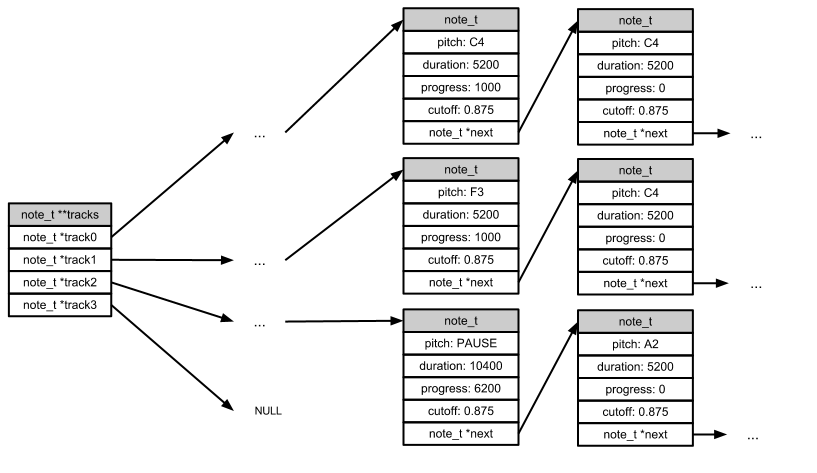
\includegraphics[width=480px]{tracks_example02.png}}}
	\caption{Example of what the tracks array in \textbf{playback.c} may look like}
	\label{tracks-example}
\end{figure}
During execution of the song, the \textbf{tracks} array in \textbf{playback.c}
will look something like Figure[\ref{tracks-example}].
Whenever the progress of a note\_t struct exceeds the duration of the note,
the \textbf{get\_track\_pitch} function will handle the switch
to the next note in the respective track. While one
track switches a note, the other tracks may stay on the same. \\
\\
When all the tracks have reached the end of the linked list we tried to implement a
stop action to turn of the ABDAC (as is done between notes in the piano). This implementation
did not work. But we recognize this is a vital part of a energy efficient system.

  \subsection{Drivers}
The led driver and the button driver has a lot of similar code, mainly 
the initialization process and the termination process of the driver. 
They are both character devices that registers a memory region on the 
PIOB and registers itself as a character device, with major numbers and 
file operations like read and write. The following sections 
describe the implementation of the led driver, but the procedure is equal for the buttons driver.

\subsubsection{Module initialization}
The leds and buttons driver have the init functions \textbf{leds\_init}
and \textbf{buttons\_init}, respectively. They are registered, and thus 
picked up by the kernel, by calling the function \textbf{module\_init}
passing the init-function as a parameter.
\\
\begin{lstlisting}
module_init ( leds_init );
\end{lstlisting}
Both the drivers have a file\_operations structure,
defined in the C file. All it does is map different file operations,
implemented in the driver, to the ones defined in the structure.
This file\_operations structure will later on be registered together
with the actual device.
\\
\begin{lstlisting}
static struct file_operations led_fops = {
	.owner = THIS_MODULE,
	.open = open_leds,
	.write = write_leds,
	.read = read_leds,
	.release = release_leds
};
\end{lstlisting}
The first thing that happens inside the leds\_init function
is allocation of a character device region
and assigning a major number to the device.
\\
\begin{lstlisting}
static int leds_init ( void ) {
	//...
	result = alloc_chrdev_region ( &dev, leds_minor, 
		NUM_DEVICES, "leds" );
	leds_major = MAJOR ( dev );
	//...
\end{lstlisting}
If alloc\_chrdev\_region returns a negative number there is a problem getting
a major number to the device and the init method returns with an error.
If result is positive we build a dev\_t data item, 
representing the device based on the minor and major number, and requests memory region that we are going to use on the GPIO at the PIOB address.
If all goes well we initialize the \textit{per} and, 
\textit{oer} registers at piob (\textit{per} and \textit{puer}
for buttons), in order to be able to read and write from PIOB.
\\
\begin{lstlisting}
dev = MKDEV ( leds_major, leds_minor );
result = (int) request_region ( AVR32_PIOB_ADDRESS, mem_quantum, "leds" );
// Initialize the leds
volatile avr32_pio_t *piob = &AVR32_PIOB;
piob->per |= 0xff;
piob->oer |= 0xff;
\end{lstlisting}
Finally, the leds\_init function allocates and sets up the character 
device structure \textit{char\_dev}. 
It adds all the led file operations defined in
the struct \textit{led\_fops} to \textit{char\_dev}, and 
it registers the device with the dev\_t \textit{dev} data item.
\\
\begin{lstlisting}
// Set up char_dev structure for the device
struct cdev *char_dev = cdev_alloc ();
cdev_init ( char_dev, &led_fops );
char_dev->owner = THIS_MODULE;
char_dev->ops = &led_fops;
int error = cdev_add (char_dev, dev, 1);
\end{lstlisting}
If there is an error, i.e. \textit{error} is a positive number, it will
be logged to the kernel. Otherwise, the device driver initialization 
should have completed successfully.

\subsubsection{Module termination}
The drivers also have an exit-function, \textbf{leds\_exit} and 
\textbf{buttons\_exit} that is registered the same way as 
the init function. This function is called when the kernel module is 
removed from the operating system. 
\\
\begin{lstlisting}
module_exit ( leds_exit );
\end{lstlisting}
The termination procedure of the kernel module is much smaller than the 
initialization procedure. It basically clears out the output register
on the device, releases the previously requested memory region and
unregisters the previously registered character device region for
the device.
\\
\begin{lstlisting}
static void leds_exit ( void ) {
	int mem_quantum = sizeof( avr32_pio_t );
	volatile avr32_pio_t *piob = &AVR32_PIOB;
	piob->codr = 0xff;
	release_region ( AVR32_PIOB_ADDRESS, mem_quantum );
	unregister_chrdev_region ( dev, NUM_DEVICES );
}
\end{lstlisting}


  \subsection{Led Driver}
%\label{sec:result}
To test the led driver we wrote a simple c program that did three things;
\begin{enumerate}
  \item Initialize the leds, i.e. open the file \textit{/dev/leds} with write permission
  \item Write different values to the led
  \item Close the file
\end{enumerate}
The simple test is testing one light at the time, before it pauses for one secound and 
lights the next one.\\
\\
{\bf Test Case 1}: Open leds through a C program \\
{\bf Description}: It should be possible to open and close the device file through a
C program \\
{\bf Precondition}: Board is set up with operating system and the drivers are loaded\\
{\bf Execution}: Run the program, calling the {\it open(file, flag)} function on the device
file., followed by a {\it close} on the file.\\
{\bf Expected Result}: {\it open} should NOT return a negative number, {\it close}
should return 0.\\
{\bf Observed Result}: {\it open} returned a positive number, {\it close}
returned 0. \\
 \\
{\bf Test Case 2}: Write to leds through a C program. LED 0 should light \\
{\bf Description}: The first lED should be on after writing to the device file \\
{\bf Precondition}: Board is set up with operating system and the drivers are loaded,
and device file is opened with the {\it O\_WRONLY} flag.\\
{\bf Execution}: Write the {\it short int} value 1 to the device file \\
{\bf Expected Result}: LED 0 should be ON, all other leds should be OFF. \\
{\bf Observed Result}: LED 0 was the only active LED \\
 \\
{\bf Test Case 3}: Write to leds through the linux terminal\\
{\bf Description}: Write a single byte to the device file using a terminal commando\\
{\bf Precondition}: Board is set up with operating system and the drivers are loaded\\
{\bf Execution}: Run the command {\bf echo A > /dev/leds} \\
{\bf Expected Result}: LED 6 and LED 0 should be ON, all other leds should be OFF.\\
{\bf Observed Result}: LED 6 and LED 0 turned ON, the others turned OFF. We also
observed that the command did not end the execution in the terminal.\\
 \\
There was one problem with the third test case. The exectued command did not seam to end.
While looking over the kernel logs we found that the value {\it 10}, the ascii value for
{\it new line}, was constantly being tried written to the device file. Thus it seams like
the driver is not working fully as expected, but it serves its purpose when writing to it 
through a C program.
  \subsection{Button Driver}
The init function of the buttons driver sets up the buttons in the same way as the previous exercise, in addition to the general procedure for the drivers described above. The buttons are only using half of the pins, the rest are used by the LEDs, the issue of disabling/enabling buttons and not LEDs is solved by OR-ing the current value with ff00:
\\
\begin{lstlisting}
piob->per |= 0xff00;
piob->puer |= 0xff00;
\end{lstlisting}
The buttons driver has, unlike the LEDs driver, a read-function. The read function provides the ability to read the status of the buttons. The status is read from PDSR of the memory map region of PIOB. The status of the pins are however not located in a sequential order. This is handled by a sequence of if sentences that accumulates the status in a proper sequential bitmap, where the first bit represents the left most button and the last bit represents the right most button. The result is written to the output buffer.\\
\\
Interrupts were also implemented in the buttons driver but is not part of the final game. To enable interrupts each of the buttons were registered with an IRQ, and the buttons\_interrupt method to handle the interrupts. The IER register in PIOB was set to 1 as in the previous exercise.
\\
\begin{lstlisting}
piob->ier = 0xff00;
const int pins[8] = {40, 41, 42, 45, 46, 47, 48, 62};
int i;
for (i=0; i < 8; i++) {
	// Request IRQ
	irqs[i] = gpio_to_irq(pins[i]);
	result = request_irq(irqs[i], button_interrupt, 0, "buttons", NULL);
	if (result){
		printk(KERN_ALERT "error %d: could not request irq: %d\n", result, irqs[i] , pins[i]);
		return result;
	}else{
		printk(KERN_ALERT "requested pin %d with irq: %d\n", pins[i], irqs[i]);
	}
}
\end{lstlisting}
In the button\_exit function the IRQs are freed:
\\
\begin{lstlisting}
int i;
for (i = 0; i < 8; i++) {
	printk(KERN_ALERT "exit : removing irq: %d\n",irqs[i]);
	free_irq(irqs[i],  NULL);
}
\end{lstlisting}
The interrupt routine in buttons\_interrupt simply prints a message telling which button was pressed, based on the IRQ:
\\
\begin{lstlisting}
static irqreturn_t button_interrupt(int irq, void *dev_id)
{
	if (irq == irqs[0]) {
		if (callbacks_struct.cb1) { (*callbacks_struct.cb1)(); }
		printk(KERN_ALERT "interrupt from sw%d", 0);
	}else if (irq == irqs[1]) {
		printk(KERN_ALERT "interrupt from sw%d", 1);
	}else if (irq == irqs[2]) {
		printk(KERN_ALERT "interrupt from sw%d", 2);
	}else if (irq == irqs[3]) {
		printk(KERN_ALERT "interrupt from sw%d", 3);
	}else if (irq == irqs[4]) {
		printk(KERN_ALERT "interrupt from sw%d", 4);
	}else if (irq == irqs[5]) {
		printk(KERN_ALERT "interrupt from sw%d", 5);
	}else if (irq == irqs[6]) {
		printk(KERN_ALERT "interrupt from sw%d", 6);
	}else if (irq == irqs[7]) {
		printk(KERN_ALERT "interrupt from sw%d", 7);
	}
	return IRQ_HANDLED;
}
\end{lstlisting}
To use interrupts in the game, the button\_interrupt function could send a callback to the game when interrupts occurs. The callback could be registered in the driver through a IOCTL function. But, as stated earlier, we did not implement this part in the final solution, due to lack of time.

  \subsection{Graphics}

\subsubsection{Screen}

The screen is opened and memory mapped in the {\bf Screen} object like this.
\\
\begin{lstlisting}
  int fd = screen->_fd = open( "/dev/fb0", ... );
  screen->frame_buffer = (uint8_t*)mmap( 0, SCREEN_SIZE, ... , MAP_SHARED, fd, 0 );
\end{lstlisting}
The screen has a method {\bf ScreenFlush} to flush the whole internal buffer into the frame buffer:
\\
\begin{lstlisting}
  void ScreenFlush( Screen *screen ) {

    for (int i=0; i < SCREEN_SIZE; i++) {
      screen->frame_buffer[i] = screen->internal_buffer[i];
    }

  }
\end{lstlisting}
To draw to the internal buffer it supplies the {\bf ScreenDrawPixel} method:
\\
\begin{lstlisting}

  void ScreenDrawPixel(Screen *screen, int x, int y, Pixel *pixel) {

    if (x >= 0 && x < screen->width && y >= 0 && y < screen->height) {
      if (PixelNotTransparant(pixel)) {
	int coordinate = y * screen->width * 3 + x * 3;
	*((Pixel*)&screen->internal_buffer[coordinate]) = *pixel;
      }
    }
  }
\end{lstlisting}
The {\bf PixelNotTransparant} function lets us paint pictures with
transparency. If it returns {\bf false} the pixel is simply not drawn.
The function also does boundry checks to make sure that the pixel is
on the screen. This helps the graphical objects to not care about
whether they
are on the screen or not in their paint method.

\subsubsection{Canvas}
The {\bf CanvasPaint} method is found in the core of the {\bf Canvas} object.
It is reponsible for drawing each graphical object on to the
screen. This loop runs though all objects and ask them to paint themselves
 on the screen.
\\
\begin{lstlisting}
  for (int i=0; i<canvas->top; i++) {
    if (canvas->shapes[i]) {
      Shape *shape = (Shape*)canvas->shapes[i];

      (*((Shape*)shape)->paint)( canvas->shapes[i], screen );
    }
  }
\end{lstlisting}
Afterwards, the method asks the {\bf Screen} object to update the screen
buffer through the {\bf ScreenFlush} method.

\subsubsection{Shape}
The {\bf Shape} exists only to provide a structure for which other
graphical objects shall match. In this implementation the most
importaint part is the {\bf paint} function pointer, which all
graphical object must have as their second member. The first member is
a pointer to the objects parent. This is only used for the {\bf Bitmap}
type.
\\
\begin{lstlisting}
  typedef struct {
    void *parent;
    void (*paint) ( void*, Screen* );
    int x;
    int y;
    void *child;
  } Shape;
\end{lstlisting}

\subsubsection{Image}
The {\bf Image} object is only an abstract object, its responsibility
is to conseal the implemented file format. Therefore, its implementetion
is fairly simple. The {\bf paint} method delegates all its work to the
format specific object.
\\
\begin{lstlisting}
  static void paint (void *shape, Screen *screen) {

    Image *image = (Image*) shape;
    Shape *actual_image = (Shape*)image->image;
    actual_image->paint( actual_image, screen  );

  }
\end{lstlisting}

\subsubsection{Bitmap}
The {\bf Bitmap} object is by far the most complex object in the
graphics module. It is responsible for reading the bitmap fileformat
and rendering its contents in the internal buffer. The reading is
implemented in three steps.

\begin{enumerate}
\item Reading the file header \newline
  The file header is read directly into the {\bf BMPHeader} structure.
  \begin{lstlisting}
    static BMPHeader ReadBMPHeader ( int fd ) {

      BMPHeader header;
      read( fd, &header, sizeof(header));

      return header;
    }
  \end{lstlisting}

\item Reading the DIB header \newline
  We only need the first three fields of the DIB header, these are read
  into the struct.
  \begin{lstlisting}
    static DIBHeader ReadDIBHeader ( int fd ) {

      DIBHeader header;
      read( fd, &header, sizeof(header));
      return header;
    }
  \end{lstlisting}

\item Converting endian of the file header \newline
  The fileformat headers are written in little-endian, the Linux on the
  board uses big-endian. This is fixed with a bit of byte swapping.
  \begin{lstlisting}
    static void fix_endian( BMPHeader *bmp_header, DIBHeader *dib_header ) {

      char *p;

      // BMP header
      p = (char*) &bmp_header->signature;
      swap( &p[0], &p[1] );

      p = (char*) &bmp_header->size;
      swap( &p[0], &p[3] );
      swap( &p[1], &p[2] );

      p = (char*) &bmp_header->reserved1;
      swap( &p[0], &p[1] );

      p = (char*) &bmp_header->reserved1;
      swap( &p[0], &p[1] );

      p = (char*) &bmp_header->offset;
      swap( &p[0], &p[3] );
      swap( &p[1], &p[2] );

      // DIB header
      p = (char*) &dib_header->size;
      swap( &p[0], &p[3] );
      swap( &p[1], &p[2] );

      p = (char*) &dib_header->width;
      swap( &p[0], &p[3] );
      swap( &p[1], &p[2] );

      p = (char*) &dib_header->height;
      swap( &p[0], &p[3] );
      swap( &p[1], &p[2] );

    }
  \end{lstlisting}

\item Making sense of the headers
  \begin{lstlisting}
    int offset = bmp_header.offset;
    int size = bmp_header.size;
    int width = dib_header.width;
    int height = dib_header.height;
  \end{lstlisting}
\item Reading the content \newline
  The actual bitmap from the offset in the header untill the end of the
  file. All of this is read into the {\bf data} variable.
  \begin{lstlisting}
    uint8_t *data = malloc(size);
    uint8_t *ptr = (uint8_t*)data;

    for (int i=0; i < (size - offset) / BUFFER_SIZE; i++ ) {
      read( fd, buffer, BUFFER_SIZE );

      for (int i=0; i<BUFFER_SIZE; i++) {
	(*ptr++) = buffer[i];
      }
    }

    int remaining = (size - offset) % BUFFER_SIZE;
    if (remaining) {
      read( fd, buffer, remaining);

      for (int i=0; i<remaining; i++) {

	(*ptr++) = buffer[i];
      }
    }
  \end{lstlisting}

  \item Flipping the rows of the content \newline
The rows in the bitmap array is stored in the wrong order so
we have to flip them over.
    \begin{lstlisting}
      static void swapLine ( uint8_t *a, uint8_t *b, int width ) {

	for (int i=0; i<width; i++) {
	  swap(&a[i], &b[i]);
	}

      for (int i=0; i<width; i++) {
	swap(&a[i], &b[i]);
      }

    }

    static void flip ( uint8_t *data, int width, int height ) {

      for (int i=0, j=height-1 ; i < height/2; i += 1, j -= 1) {
	swapLine( &data[i*width*3], &data[j*width*3], width*3 );
      }
    \end{lstlisting}
  \item Saving the useful data\newline
Now we only need the {\bf width}, {\bf height} and {\bf data} in order
to draw the image on the screen.
    \begin{lstlisting}
	bmp->width = width;
	bmp->height = height;
	bmp->pixels = data;
    \end{lstlisting}
\end{enumerate}
The {\bf paint} method of the {\bf Bitmap} object copies the pixel
values from its internal memory. It draws them on the screen with a
vertical and horizontal shift according to its parent, {\bf Image}, x
and y values. This enables the image to be painted at an arbitrary
place on the screen.
\\
\begin{lstlisting}
  static void paint ( void *shape, Screen *screen ) {

    Bitmap *image = (Bitmap*) shape;
    Image *parent = (Image*) image->parent;

    int sx = parent->x;
    int sy = parent->y;

    int width = image->width;
    int height = image->height;

    for (int y = 0; y < height; y++) {
      for (int x = 0; x < width; x++) {
	Pixel *p = &image->pixels[y*width + x];
	ScreenDrawPixel( screen, x+sx, y+sy, p);
      }
    }
  }
\end{lstlisting}

\subsubsection{Line}
The {\bf Line} object is responsible for drawing lines on the {\bf Screen}. It can be
used for making compound objects like rectangles and triangles. The paint method uses
Simplified Bresenham's line algorithm\footnote{http://en.wikipedia.org/wiki/Bresenham's\_line\_algorithm}.

\begin{lstlisting}
  while (1) {
    ScreenDrawPixel(screen, x0, y0, &pixel);
    if (x0 == x1 && y0 == y1) {
      break;
    }

    int e2 = 2*err;
    if (e2 > -dy) {
      err = err - dy;
      x0 = x0 + sx;
    }
    if (e2 < dy) {
      err = err + dx;
      y0 = y0 + sy;
    }
  }

\end{lstlisting}

\subsubsection{Rectangle}
The {\bf Rectangle} object uses the {\bf Line} object to draw a rectangle on the {\bf Screen}.
\begin{lstlisting}
  static void paint ( void *shape, Screen *screen ) {

    Rectangle *rect = (Rectangle*)shape;

    int x = rect->x;
    int y = rect->y;
    int dx = rect->dx;
    int dy = rect->dy;

    Line l1 = LineNew(x, y, dx, 0);
    l1.paint( &l1, screen );

    Line l2 = LineNew(x, y+dy, dx, 0);
    l2.paint( &l2, screen );

    Line l3 = LineNew(x, y, 0, dy);
    l3.paint( &l3, screen );

    Line l4 = LineNew(x+dx, y, 0, dy);
    l4.paint( &l4, screen );
  }
\end{lstlisting}

  \subsection{Sound}
\label{sec:alsa}

In order to have audible sound on the board the sound setting in Linux must be set correctly.

This can be done by opening the alsamixer (execute {\bf alsamixer} as root at the shell prompt).
Here all items should be unmuted, select the item with the arrows and unmute with the {\bf m} key.
The items must also be set to appropiate levels, the levels are set with the arrow keys. Exit
the program with the {\bf ESC} key.

  \subsection{Game}
The game was simply tested during development, the iterative process of implementing
small parts and testing them, eventually led to a fully working game. There are 
mainly three things that should work;
\begin{enumerate}
  \item Player A should be able to move the tank
  \item Player B should be able to move the cannon aim
  \item The round should end in favour to player A if the tank reaches the turret, or it
  	should end in favour to player B if the turret hits the tank.
\end{enumerate}

\subsubsection{Tank movement}
The tank should be able to move in all four directions, and accross the whole field. The only 
restrictions is when trying to move out of the field (the bounds of the game) and when
trying to move over fire. When the tank enters the top right tile, i.e. the location of the 
turret, the round should end in favour to the tank. Thus the tank can find itself in four
different situations;
\begin{enumerate}
  \item Trying to move over open field
  \item Trying to move over fire
  \item Trying to move out of the field
  \item Trying to move on top of the turret
\end{enumerate}

\subsubsection{Turret movement}
The turret does not have the same controls as the tank, but it beahves almost the same. 
The main difference is the possibility to shoot anything execpt for itself. 
The turret can find itself in three different situations.
\begin{enumerate}
  \item Trying to aim over open field
  \item Trying to aim out of the field
  \item Shoot where it aims. It should not have any effect if it tries to shoot at fire
  or itself.
\end{enumerate}

\subsubsection{Ending the game}
A round should end when either player A has reached the turret, or player B has hit the tank.
Each player has four lives indicated by how many lights are lighting. When one player has won
four rounds the player should also have won the game (making the other player a looser), 
and the screen should display two different images depending on who won the game. There are
two different scenarios;
\begin{enumerate}
  \item Player A wins
  \item Player B wins
\end{enumerate}

\subsubsection{Test results}
We have tested all the previously listed situations for tank and turret, from two to four
different angles (depending on edges and corners of the field), and they all work
according to the expectations. \\
\\
We have also tested playing the game by winning four consecutive turns for player A and for 
player B, and we have tested different combinations of winning and losing rounds. 
The lights represenenting the remaining lives work as expected, and the game ends displaying
the correct image after a player has won four rounds.

  \include*{testreport}
  \include*{testreport/leddriver}
  \subsection{Button Driver}
The init function of the buttons driver sets up the buttons in the same way as the previous exercise, in addition to the general procedure for the drivers described above. The buttons are only using half of the pins, the rest are used by the LEDs, the issue of disabling/enabling buttons and not LEDs is solved by OR-ing the current value with ff00:
\\
\begin{lstlisting}
piob->per |= 0xff00;
piob->puer |= 0xff00;
\end{lstlisting}
The buttons driver has, unlike the LEDs driver, a read-function. The read function provides the ability to read the status of the buttons. The status is read from PDSR of the memory map region of PIOB. The status of the pins are however not located in a sequential order. This is handled by a sequence of if sentences that accumulates the status in a proper sequential bitmap, where the first bit represents the left most button and the last bit represents the right most button. The result is written to the output buffer.\\
\\
Interrupts were also implemented in the buttons driver but is not part of the final game. To enable interrupts each of the buttons were registered with an IRQ, and the buttons\_interrupt method to handle the interrupts. The IER register in PIOB was set to 1 as in the previous exercise.
\\
\begin{lstlisting}
piob->ier = 0xff00;
const int pins[8] = {40, 41, 42, 45, 46, 47, 48, 62};
int i;
for (i=0; i < 8; i++) {
	// Request IRQ
	irqs[i] = gpio_to_irq(pins[i]);
	result = request_irq(irqs[i], button_interrupt, 0, "buttons", NULL);
	if (result){
		printk(KERN_ALERT "error %d: could not request irq: %d\n", result, irqs[i] , pins[i]);
		return result;
	}else{
		printk(KERN_ALERT "requested pin %d with irq: %d\n", pins[i], irqs[i]);
	}
}
\end{lstlisting}
In the button\_exit function the IRQs are freed:
\\
\begin{lstlisting}
int i;
for (i = 0; i < 8; i++) {
	printk(KERN_ALERT "exit : removing irq: %d\n",irqs[i]);
	free_irq(irqs[i],  NULL);
}
\end{lstlisting}
The interrupt routine in buttons\_interrupt simply prints a message telling which button was pressed, based on the IRQ:
\\
\begin{lstlisting}
static irqreturn_t button_interrupt(int irq, void *dev_id)
{
	if (irq == irqs[0]) {
		if (callbacks_struct.cb1) { (*callbacks_struct.cb1)(); }
		printk(KERN_ALERT "interrupt from sw%d", 0);
	}else if (irq == irqs[1]) {
		printk(KERN_ALERT "interrupt from sw%d", 1);
	}else if (irq == irqs[2]) {
		printk(KERN_ALERT "interrupt from sw%d", 2);
	}else if (irq == irqs[3]) {
		printk(KERN_ALERT "interrupt from sw%d", 3);
	}else if (irq == irqs[4]) {
		printk(KERN_ALERT "interrupt from sw%d", 4);
	}else if (irq == irqs[5]) {
		printk(KERN_ALERT "interrupt from sw%d", 5);
	}else if (irq == irqs[6]) {
		printk(KERN_ALERT "interrupt from sw%d", 6);
	}else if (irq == irqs[7]) {
		printk(KERN_ALERT "interrupt from sw%d", 7);
	}
	return IRQ_HANDLED;
}
\end{lstlisting}
To use interrupts in the game, the button\_interrupt function could send a callback to the game when interrupts occurs. The callback could be registered in the driver through a IOCTL function. But, as stated earlier, we did not implement this part in the final solution, due to lack of time.

  \subsection{Graphics}

\subsubsection{Screen}

The screen is opened and memory mapped in the {\bf Screen} object like this.
\\
\begin{lstlisting}
  int fd = screen->_fd = open( "/dev/fb0", ... );
  screen->frame_buffer = (uint8_t*)mmap( 0, SCREEN_SIZE, ... , MAP_SHARED, fd, 0 );
\end{lstlisting}
The screen has a method {\bf ScreenFlush} to flush the whole internal buffer into the frame buffer:
\\
\begin{lstlisting}
  void ScreenFlush( Screen *screen ) {

    for (int i=0; i < SCREEN_SIZE; i++) {
      screen->frame_buffer[i] = screen->internal_buffer[i];
    }

  }
\end{lstlisting}
To draw to the internal buffer it supplies the {\bf ScreenDrawPixel} method:
\\
\begin{lstlisting}

  void ScreenDrawPixel(Screen *screen, int x, int y, Pixel *pixel) {

    if (x >= 0 && x < screen->width && y >= 0 && y < screen->height) {
      if (PixelNotTransparant(pixel)) {
	int coordinate = y * screen->width * 3 + x * 3;
	*((Pixel*)&screen->internal_buffer[coordinate]) = *pixel;
      }
    }
  }
\end{lstlisting}
The {\bf PixelNotTransparant} function lets us paint pictures with
transparency. If it returns {\bf false} the pixel is simply not drawn.
The function also does boundry checks to make sure that the pixel is
on the screen. This helps the graphical objects to not care about
whether they
are on the screen or not in their paint method.

\subsubsection{Canvas}
The {\bf CanvasPaint} method is found in the core of the {\bf Canvas} object.
It is reponsible for drawing each graphical object on to the
screen. This loop runs though all objects and ask them to paint themselves
 on the screen.
\\
\begin{lstlisting}
  for (int i=0; i<canvas->top; i++) {
    if (canvas->shapes[i]) {
      Shape *shape = (Shape*)canvas->shapes[i];

      (*((Shape*)shape)->paint)( canvas->shapes[i], screen );
    }
  }
\end{lstlisting}
Afterwards, the method asks the {\bf Screen} object to update the screen
buffer through the {\bf ScreenFlush} method.

\subsubsection{Shape}
The {\bf Shape} exists only to provide a structure for which other
graphical objects shall match. In this implementation the most
importaint part is the {\bf paint} function pointer, which all
graphical object must have as their second member. The first member is
a pointer to the objects parent. This is only used for the {\bf Bitmap}
type.
\\
\begin{lstlisting}
  typedef struct {
    void *parent;
    void (*paint) ( void*, Screen* );
    int x;
    int y;
    void *child;
  } Shape;
\end{lstlisting}

\subsubsection{Image}
The {\bf Image} object is only an abstract object, its responsibility
is to conseal the implemented file format. Therefore, its implementetion
is fairly simple. The {\bf paint} method delegates all its work to the
format specific object.
\\
\begin{lstlisting}
  static void paint (void *shape, Screen *screen) {

    Image *image = (Image*) shape;
    Shape *actual_image = (Shape*)image->image;
    actual_image->paint( actual_image, screen  );

  }
\end{lstlisting}

\subsubsection{Bitmap}
The {\bf Bitmap} object is by far the most complex object in the
graphics module. It is responsible for reading the bitmap fileformat
and rendering its contents in the internal buffer. The reading is
implemented in three steps.

\begin{enumerate}
\item Reading the file header \newline
  The file header is read directly into the {\bf BMPHeader} structure.
  \begin{lstlisting}
    static BMPHeader ReadBMPHeader ( int fd ) {

      BMPHeader header;
      read( fd, &header, sizeof(header));

      return header;
    }
  \end{lstlisting}

\item Reading the DIB header \newline
  We only need the first three fields of the DIB header, these are read
  into the struct.
  \begin{lstlisting}
    static DIBHeader ReadDIBHeader ( int fd ) {

      DIBHeader header;
      read( fd, &header, sizeof(header));
      return header;
    }
  \end{lstlisting}

\item Converting endian of the file header \newline
  The fileformat headers are written in little-endian, the Linux on the
  board uses big-endian. This is fixed with a bit of byte swapping.
  \begin{lstlisting}
    static void fix_endian( BMPHeader *bmp_header, DIBHeader *dib_header ) {

      char *p;

      // BMP header
      p = (char*) &bmp_header->signature;
      swap( &p[0], &p[1] );

      p = (char*) &bmp_header->size;
      swap( &p[0], &p[3] );
      swap( &p[1], &p[2] );

      p = (char*) &bmp_header->reserved1;
      swap( &p[0], &p[1] );

      p = (char*) &bmp_header->reserved1;
      swap( &p[0], &p[1] );

      p = (char*) &bmp_header->offset;
      swap( &p[0], &p[3] );
      swap( &p[1], &p[2] );

      // DIB header
      p = (char*) &dib_header->size;
      swap( &p[0], &p[3] );
      swap( &p[1], &p[2] );

      p = (char*) &dib_header->width;
      swap( &p[0], &p[3] );
      swap( &p[1], &p[2] );

      p = (char*) &dib_header->height;
      swap( &p[0], &p[3] );
      swap( &p[1], &p[2] );

    }
  \end{lstlisting}

\item Making sense of the headers
  \begin{lstlisting}
    int offset = bmp_header.offset;
    int size = bmp_header.size;
    int width = dib_header.width;
    int height = dib_header.height;
  \end{lstlisting}
\item Reading the content \newline
  The actual bitmap from the offset in the header untill the end of the
  file. All of this is read into the {\bf data} variable.
  \begin{lstlisting}
    uint8_t *data = malloc(size);
    uint8_t *ptr = (uint8_t*)data;

    for (int i=0; i < (size - offset) / BUFFER_SIZE; i++ ) {
      read( fd, buffer, BUFFER_SIZE );

      for (int i=0; i<BUFFER_SIZE; i++) {
	(*ptr++) = buffer[i];
      }
    }

    int remaining = (size - offset) % BUFFER_SIZE;
    if (remaining) {
      read( fd, buffer, remaining);

      for (int i=0; i<remaining; i++) {

	(*ptr++) = buffer[i];
      }
    }
  \end{lstlisting}

  \item Flipping the rows of the content \newline
The rows in the bitmap array is stored in the wrong order so
we have to flip them over.
    \begin{lstlisting}
      static void swapLine ( uint8_t *a, uint8_t *b, int width ) {

	for (int i=0; i<width; i++) {
	  swap(&a[i], &b[i]);
	}

      for (int i=0; i<width; i++) {
	swap(&a[i], &b[i]);
      }

    }

    static void flip ( uint8_t *data, int width, int height ) {

      for (int i=0, j=height-1 ; i < height/2; i += 1, j -= 1) {
	swapLine( &data[i*width*3], &data[j*width*3], width*3 );
      }
    \end{lstlisting}
  \item Saving the useful data\newline
Now we only need the {\bf width}, {\bf height} and {\bf data} in order
to draw the image on the screen.
    \begin{lstlisting}
	bmp->width = width;
	bmp->height = height;
	bmp->pixels = data;
    \end{lstlisting}
\end{enumerate}
The {\bf paint} method of the {\bf Bitmap} object copies the pixel
values from its internal memory. It draws them on the screen with a
vertical and horizontal shift according to its parent, {\bf Image}, x
and y values. This enables the image to be painted at an arbitrary
place on the screen.
\\
\begin{lstlisting}
  static void paint ( void *shape, Screen *screen ) {

    Bitmap *image = (Bitmap*) shape;
    Image *parent = (Image*) image->parent;

    int sx = parent->x;
    int sy = parent->y;

    int width = image->width;
    int height = image->height;

    for (int y = 0; y < height; y++) {
      for (int x = 0; x < width; x++) {
	Pixel *p = &image->pixels[y*width + x];
	ScreenDrawPixel( screen, x+sx, y+sy, p);
      }
    }
  }
\end{lstlisting}

\subsubsection{Line}
The {\bf Line} object is responsible for drawing lines on the {\bf Screen}. It can be
used for making compound objects like rectangles and triangles. The paint method uses
Simplified Bresenham's line algorithm\footnote{http://en.wikipedia.org/wiki/Bresenham's\_line\_algorithm}.

\begin{lstlisting}
  while (1) {
    ScreenDrawPixel(screen, x0, y0, &pixel);
    if (x0 == x1 && y0 == y1) {
      break;
    }

    int e2 = 2*err;
    if (e2 > -dy) {
      err = err - dy;
      x0 = x0 + sx;
    }
    if (e2 < dy) {
      err = err + dx;
      y0 = y0 + sy;
    }
  }

\end{lstlisting}

\subsubsection{Rectangle}
The {\bf Rectangle} object uses the {\bf Line} object to draw a rectangle on the {\bf Screen}.
\begin{lstlisting}
  static void paint ( void *shape, Screen *screen ) {

    Rectangle *rect = (Rectangle*)shape;

    int x = rect->x;
    int y = rect->y;
    int dx = rect->dx;
    int dy = rect->dy;

    Line l1 = LineNew(x, y, dx, 0);
    l1.paint( &l1, screen );

    Line l2 = LineNew(x, y+dy, dx, 0);
    l2.paint( &l2, screen );

    Line l3 = LineNew(x, y, 0, dy);
    l3.paint( &l3, screen );

    Line l4 = LineNew(x+dx, y, 0, dy);
    l4.paint( &l4, screen );
  }
\end{lstlisting}

  \subsection{Sound}
\label{sec:alsa}

In order to have audible sound on the board the sound setting in Linux must be set correctly.

This can be done by opening the alsamixer (execute {\bf alsamixer} as root at the shell prompt).
Here all items should be unmuted, select the item with the arrows and unmute with the {\bf m} key.
The items must also be set to appropiate levels, the levels are set with the arrow keys. Exit
the program with the {\bf ESC} key.

  \subsection{Game}
The game was simply tested during development, the iterative process of implementing
small parts and testing them, eventually led to a fully working game. There are 
mainly three things that should work;
\begin{enumerate}
  \item Player A should be able to move the tank
  \item Player B should be able to move the cannon aim
  \item The round should end in favour to player A if the tank reaches the turret, or it
  	should end in favour to player B if the turret hits the tank.
\end{enumerate}

\subsubsection{Tank movement}
The tank should be able to move in all four directions, and accross the whole field. The only 
restrictions is when trying to move out of the field (the bounds of the game) and when
trying to move over fire. When the tank enters the top right tile, i.e. the location of the 
turret, the round should end in favour to the tank. Thus the tank can find itself in four
different situations;
\begin{enumerate}
  \item Trying to move over open field
  \item Trying to move over fire
  \item Trying to move out of the field
  \item Trying to move on top of the turret
\end{enumerate}

\subsubsection{Turret movement}
The turret does not have the same controls as the tank, but it beahves almost the same. 
The main difference is the possibility to shoot anything execpt for itself. 
The turret can find itself in three different situations.
\begin{enumerate}
  \item Trying to aim over open field
  \item Trying to aim out of the field
  \item Shoot where it aims. It should not have any effect if it tries to shoot at fire
  or itself.
\end{enumerate}

\subsubsection{Ending the game}
A round should end when either player A has reached the turret, or player B has hit the tank.
Each player has four lives indicated by how many lights are lighting. When one player has won
four rounds the player should also have won the game (making the other player a looser), 
and the screen should display two different images depending on who won the game. There are
two different scenarios;
\begin{enumerate}
  \item Player A wins
  \item Player B wins
\end{enumerate}

\subsubsection{Test results}
We have tested all the previously listed situations for tank and turret, from two to four
different angles (depending on edges and corners of the field), and they all work
according to the expectations. \\
\\
We have also tested playing the game by winning four consecutive turns for player A and for 
player B, and we have tested different combinations of winning and losing rounds. 
The lights represenenting the remaining lives work as expected, and the game ends displaying
the correct image after a player has won four rounds.

  \include*{discussion}
  \include*{conclusion}
  \include*{references}

\end{document}
